
\newpage 
\section{Embedding policy, practice and supports to advance professional, managerial and support staff careers}
\label{sec:pms}

Professional, Managerial, and Support (PMS) staff as discussed in this section also includes research support staff, i.e. members of staff who perform primarily administrative tasks. 


\subsection{Reflecting on recruitment practices in the department, answer the following:}

\instr{
\begin{prompt}
\setlength\tabcolsep{6pt} 
\begin{tabu} to \textwidth { X[8] X X }    
     \multirow{2}{=}{Recruitment to PMS posts in the department adheres to institutional policy on recruitment, which includes gender-balanced panels and training for assessors.} & \textbf{Yes} & \textbf{No}  \\
     &  \XBox & \Square  \\ 
\end{tabu}
\setlength\tabcolsep{0pt} 
\end{prompt}

If you answered ‘no’, please comment.
}




\subsection{Provide three years of data on application, shortlist, and appointment rates for recruitment by gender and grade. Where data suggests opportunity for improvement, comment and reflect. Include any other relevant information relating to recruitment processes and practice for professional, managerial and support staff in the department.}



Gender specific data for selection committees and applications for the process of appointing PMS staff were not available at the time of application. However, partial records were gathered within CSIT (Tables~\ref{tab:selectioncommittee:pms}, \ref{tab:pms:appointment}). 



\begin{tabbox}{!th}
\caption[Gender composition of selection committees for PMS Appointments]{Gender composition of selection committees for PMS Appointments (2017-2020)}
\label{tab:selectioncommittee:pms}
\footnotesize 
\sisetup{
    group-digits=all,
    group-minimum-digits=4,
    group-separator = {,},
    mode=text,
    reset-text-series = false, 
    text-series-to-math = true,
    reset-text-family = false, 
    text-family-to-math = true
}
\begin{tabular}{P{2cm}
                P{6.5cm}
                C{1.3cm}
                C{1.3cm}
                !\qquad
                C{1.3cm}
                C{1.3cm}
                }
\toprule
    {Year} & 
    {Competition} & 
    \multicolumn{2}{c}{{\makecell{Chair Person}}} & 
    \multicolumn{2}{c}{{\makecell{Board Members}}} \\
    \cmidrule(l){3-4}\cmidrule(l){5-6}
    & & {F} & {M} & {F} & {M} \\
\midrule

\multicolumn{2}{l}{Administrative  (School)}\\

\midrule 
2018 & Senior Executive Assistant & 1 & 0 & 1 & 1 \\
\hdashline
2020 & Executive Assistant & 1 & 0 & 1 & 1 \\

\midrule 
\multicolumn{6}{l}{Systems Administrative  Support}\\
\midrule 

2019 & Computing Systems Engineer & 1 & 0 & 0 & 3 \\

\midrule
\multicolumn{6}{l}{Research Support}\\
\midrule

2017/18 & Systems \& HPC Lead, Insight & 1 & 0 & 2 & 4 \\

\hdashline

2018/19 & Senior Research Coordinator (EU Programme Manager), Insight & 0 & 1 & 0 & 1 \\

\cdashline{2-6}

 & Research Support Officer & * & * & * & *\\

\cdashline{2-6}

 & Senior Research Coordinator (Advance CRT Programme Manager) & 0 & 1 & 2 & 0 \\

\hdashline 

2019 /20 & Research Assistant (ADVANCE CRT) & 0 & 1 & 1 & 1  \\


\cdashline{2-6}
 & Senior Research Coordinator (CONFIRM) & 0 & 1 & 1 & 1 \\

\cdashline{2-6}

 & Research Coordinator (Insight) & 0 & 1 & 1 & 1  \\

\bottomrule
\end{tabular}
\\[2mm]
{
\footnotesize\sffamily 
* Data not available
}

\end{tabbox}





\begin{tabbox}{!th}
 
      
\footnotesize 
\caption{Recruitment of PMS staff by competition and gender (2017-2020)}
\label{tab:pms:appointment}
\sisetup{
    group-digits=all,
    group-minimum-digits=4,
    group-separator = {,},
    mode=text,
    reset-text-series = false, 
    text-series-to-math = true,
    reset-text-family = false, 
    text-family-to-math = true
}
\begin{tabular}{P{1.5cm}P{3.8cm}C{1.0cm}
                                C{1.0cm}
                                C{0.9cm}
                                !\qquad
                                C{1.0cm}
                                C{1.0cm}
                                C{0.9cm}
                                !\qquad
                                C{1.0cm}
                                C{1.0cm}}
\toprule
    {Year} & 
    {Competition} & 
    \multicolumn{3}{c}{{\makecell{Applicants}}} & 
    \multicolumn{3}{c}{{\makecell{Shortlisted}}} &
    \multicolumn{2}{c}{{\makecell{Appointed}}}\\
    \cmidrule(l){3-5}\cmidrule(l){6-8}\cmidrule(l){9-10} 
    & & {F} & {M} & {\%F} & {F} & {M} & {\%F} & {F} & {M}\\
\midrule

\multicolumn{2}{l}{Administrative  (School)}\\

\midrule 
2018 & Senior Executive Assistant & 6 & 1 & 86\% & 3 & 1 & 75\% & 0 & 1\\
\hdashline
2020 & Executive Assistant & 6 & 0 & 100\% & 4 & 0 & 100\% & 1 & 0\\

\midrule 
\multicolumn{8}{l}{Systems Administrative  Support}\\
\midrule 

2019 & Computing Systems Engineer & * & * & * & * & * & * & * & 1\\

\midrule
\multicolumn{8}{l}{Research Support}\\
\midrule

2017/18 & Systems \& HPC Lead, Insight & 0 & 1 & 0\% & 0 & 1 & 0\% & 0 & 1\\

\hdashline

2018/19 & Senior Research Coordinator (EU Programme Manager), Insight & 0 & 2 & 0\% & 0 & 1 & 0\% & 0 & 1\\

\cdashline{2-10}

%2018/19 
& Research Support Officer & 1 & 0 & 100\% & 1 & 0 & 100\% & 1 & 0\\

\cdashline{2-10}

%2018/19 
& Senior Research Coordinator (ADVANCE CRT Programme Manager) & \multicolumn{2}{c}{(8)} & -- & 2 & 2  & 0\% & 0 & 1 \\

%2019 /20 & Research Assistant (ADVANCE CRT) & 0 & 1 & 1 & 1 & 1 & 0 \\
\hdashline

2019/20 & Research Support Officer & 3 & 10 & 23\% & 3 & 10 & 23\% & 1 & 0\\

%\hdashline
% 2019 /20 & Senior Research Coordinator (CONFIRM) & 0 & 1 & 1 & 1 & 0 & 1\\

\cdashline{2-10}

%2019/20 
& Senior Research Coordinator (ADVANCE CRT) & 2 & 3 & 40\% & 2 & 3 & 40\% & 0 & 1\\

\cdashline{2-10}

%2019 /20 
& Research Coordinator (Insight) & 4 & 1 & 80\% & 4 & 1 & 80\% & {\makecell{Not\\filled}} & {\makecell{Not\\filled}} \\

\bottomrule
\end{tabular}
\\[2mm]
{
\footnotesize\sffamily 
* Data not available\\
(n) gender not recorded; total number n reported
}

\end{tabbox}




Over a three-year period, there was a relatively even distribution of genders across those shortlisted.  
There is greater gender diversity among applicants for research PMS posts. However a challenge exists in attracting a gender-diverse pool of applicants to the school office (5 F) and systems administration posts (5 M). A male staff member was recruited to the school’s administrative group in 2018 but has recently moved to a research PMS role. 
Although 12 PMS staff took the EDI survey, only 1-3 responses were received for recruitment questions. Those that answered were content with the recruitment process.

The PMS working group discussed the causation, and mechanisms to address, gender imbalance. 
These included targeted recruitment strategies and making use of a gender language software to check for bias\footnote{\url{https://capd.mit.edu/resources/gender-decoder/}} in advertisements. The new \ac{EDI} implementation committee (EDIIC) will review the language used in advertisements to provide gender-neutral language (Action~\ref{action:acad:marketing},  Page~\pageref{action:acad:marketing}).

Furthermore, the PMS workgroup discussed how to convey the EDI-friendly ethos of the school. Action~\ref{action:pms:matchdescription} was proposed to review all school materials (images and text) to convey the flexible, inclusive and collegiate nature of the school. 

Periods of leave can have a negative impact on the career of women. The workgroup discussed how this situation may have worsened since the Covid-19 pandemic. As such, Action~\ref{action:acad:cvgaps} (Page~\pageref{action:acad:cvgaps}) was proposed to invite individuals to voluntarily account for documented leave, caring responsibilities, and pandemic-related gaps in their CV. 




The PMS workgroup discussions highlighted that the advertising template for research PMS positions is the same as that for academic researchers. The standard listed application criteria are not relevant to research PMS applicants, for example, a list of publications. This may deter suitably qualified potential applicants from applying for such research PMS positions. 
In order to prevent applicant confusion regarding what research PMS roles entail, potentially limiting the pool of applicants, Action~\ref{action:pms:matchdescription} is proposed. 



\begin{actionblock}{\ksspace{}Revise PMS application forms locally}{pms:matchdescription}
\actreviewadvertisements
\hfill{
    \hypersetup{hidelinks}
    \hyperlink{d3}{\gotoactionsymbol{}}
}
\end{actionblock}


Finally, part of Action~\ref{action:enrich:opportunities} (Page~\pageref{action:enrich:opportunities}) provides an opportunity for female undergraduate students to gain relevant work experience. This includes within the school's systems administration group, which could both provide an opportunity for female undergraduates students to gain experience and introduce some gender diversity to the systems administration team. 


\subsection{Reflecting on progression in your institution, answer the following:}
\instr{
\begin{prompt}
\setlength\tabcolsep{6pt}
\begin{tabu} to \textwidth { X[8] X X }
\multirow{2}{=}{Career progression opportunities for PMS staff are centrally managed by the institution (e.g. internal vacancy competitions; regrading; promotions pathway).} & \textbf{Yes} & \textbf{No}  \\
     & {\centering \XBox } & {\centering \Square}  \\ 
\end{tabu}
\setlength\tabcolsep{0pt}
\end{prompt}

If you answered ‘no’, please comment on the department’s role in career progression for professional, managerial and support staff. 
}

All administrative promotions are handled centrally by UCC.
The EDI survey and the PMS focus group indicated that most PMS staff have no interest in career progression. Some expressed a strong dissatisfaction with the lack of progression opportunities due to infrequent promotion calls and small quotas.  

\begin{myquote}
   ``I am not familiar with the promotion scheme. It does not apply to my case and therefore I have never expressed interest on it.'' 
\end{myquote}

\begin{myquote}
   ``I think it's quite clear that this is a problem across UCC. And the unfortunate thing is, it means that UCC doesn't get the best from staff.   People that are capable of doing more are not being given the opportunity to do that, and I think that's damaging to the whole institution.''
\end{myquote}



\subsubsection{Internal vacancy competitions}
Limited opportunities exist for progressing to senior grades via internal recruitment, usually requiring a move to a different unit.  This was perceived as uncertainty and risk, since PMS staff are largely happy working within the school: 



\begin{myquote}
    ``We want to progress but [also] to remain in the School ... because, well, I'm happy here.  And in order to [be] promoted, sometimes you need to go across campus and so that puts you off a bit because, you know, your well-being and being happy [are] very important.''
\end{myquote}

\begin{myquote}
     ``Moving from [one] department in the university to another department ... can cause issues.  It's almost treated like you're starting a new job [with a period of] probation ... If you're looking for loans, mortgages, things like that ... It seems like a kind of short-sighted thing to just default onto people.''
 \end{myquote}

\subsubsection{Promotion}
PMS staff expressed strong views on the lack of promotion opportunities, which had lain dormant for a long time. In recent years regular promotional calls (every three years) have become the norm for  PMS (and Academic) staff. The first of these calls was in 2019/2020, making 53 promotional posts available. No CSIT PMS staff member applied to this scheme. Another call has recently issued for 2022/2023. 

Some female PMS staff were sceptical of the process,  believing that interviewers lacked a first hand knowledge, or understanding, of the roles that applicants occupied at the time of application.


\subsubsection{Promotion pathways}

In the survey, PMSS were asked to reflect on the career progression opportunities (Figure~\ref{fig:survey:pms:careerprogression}). Apart from one male staff member, both genders agreed that promotions are free from gender bias. 
However, 2 females and 2 males were unsure how career breaks are considered in promotion decisions. The PMS Workgroup and focus group believed that the pandemic would likely have had a negative impact on promotion. This will be addressed with Action~\ref{action:acad:cvgaps} (Page~\pageref{action:acad:cvgaps}). 


PMSS did express a desire for greater training and guidance on preparing for promotion. Given the range of diverse PMS jobs available across the university, in schools and in central administrative units, one participant felt that guidance on potential PMS career pathways within the institution would be useful, to assist staff in identifying where and how their skills and experience might be usefully redeployed and expanded. Others concurred with this view.  

PMS staff training and career development will be discussed during PDRS meetings which will restart (Action~\ref{action:acad:pdrs}).





\begin{figbox}{!ht}
    \caption{Career progression process}
    \label{fig:survey:pms:careerprogression}
    

    \sffamily
    \footnotesize
    \raggedright

    \begin{tabular}{P{3.5cm}
                    !{\quad}
                    p{10cm}}
    \addlinespace
    The promotion criteria in UCC are transparent and fair.&
    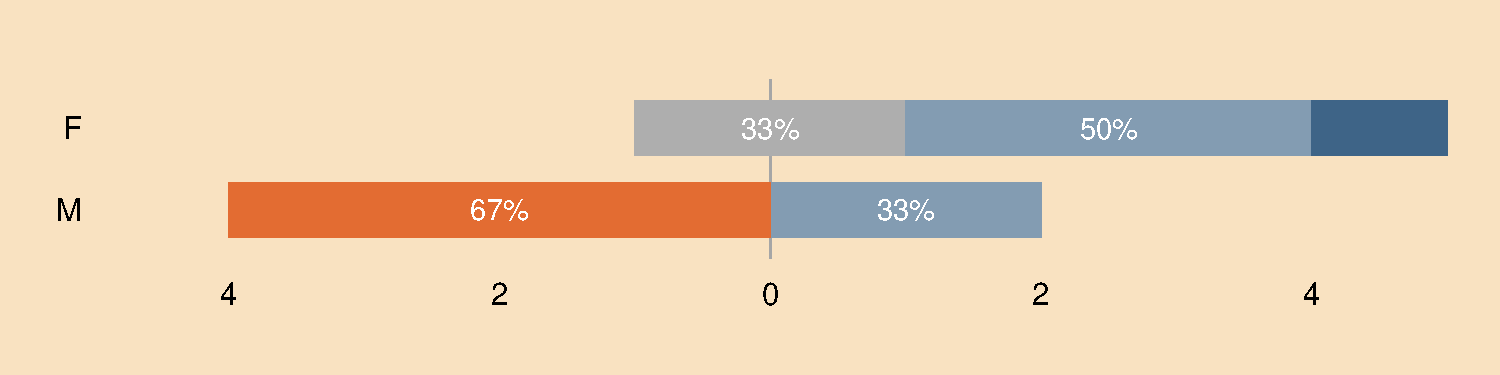
\includegraphics[align=t,trim={5mm 0 5mm 12mm},clip,width=10.5cm]{fig/pmscareer/fig231a.pdf}\\

\hdashline 

    The promotion process in UCC is transparent and fair.&
    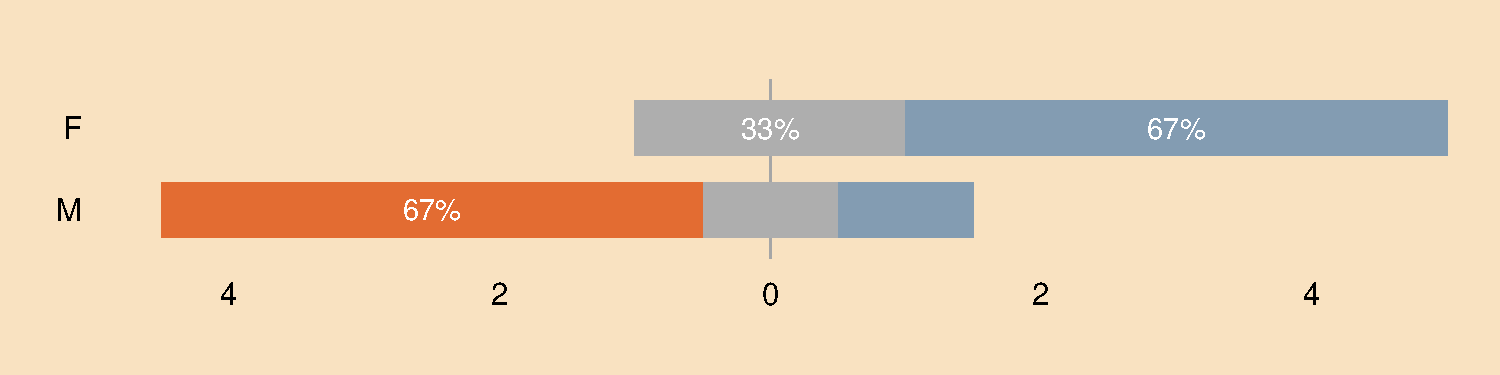
\includegraphics[align=t,trim={5mm 0 5mm 12mm},clip,width=10.5cm]{fig/pmscareer/fig231b.pdf}\\

\hdashline 

    Promotions are free of gender bias.&
    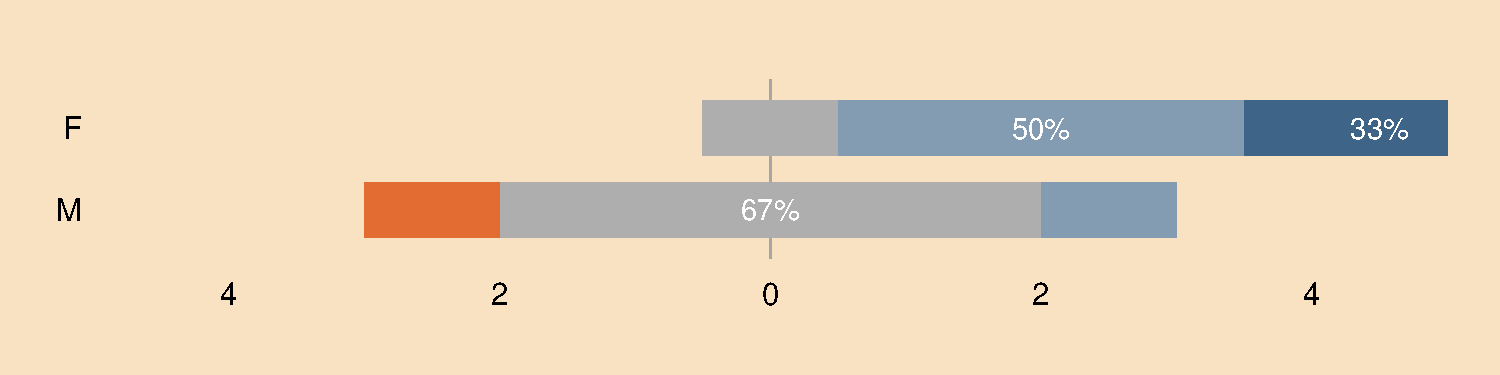
\includegraphics[align=t,trim={5mm 0 5mm 10mm},clip,width=10.5cm]{fig/pmscareer/fig231c.pdf}\\

\hdashline 

    It's clear how career breaks will be considered in promotion decisions. &
    
\includegraphics[align=t,trim={5mm 0 5mm 12mm},clip,width=10.5cm]{fig/pmscareer/fig231d.pdf}\\

\hdashline 

    Covid-19 has limited my promotion opportunities. &
    
\includegraphics[align=t,trim={5mm 0 5mm 12mm},clip,width=10.5cm]{fig/pmscareer/fig231e.pdf}\\

    %% Legend
    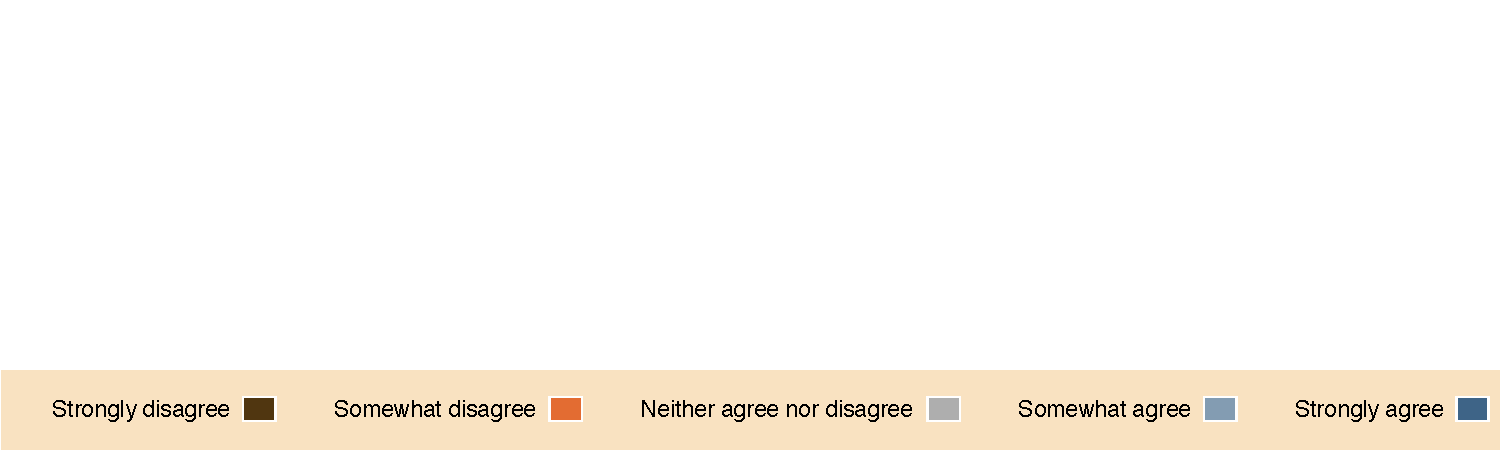
\includegraphics[trim={6mm 0 0mm 0mm},clip,width=14.5cm]{fig/legend5col.pdf}
    \end{tabular}
\end{figbox}




\newpage 
\subsection{Reflecting on opportunities for staff development review, answer the following:}

\instr{
\begin{prompt}
\setlength\tabcolsep{6pt} 
\begin{tabu} to \textwidth {@{} X[8] X X @{}}
     \multirow{2}{=}{The institution operates a development review process, or equivalent, for PMS staff} & \textbf{Yes} & \textbf{No}  \\
     &  \XBox & \Square  \\ 
\end{tabu}
\setlength\tabcolsep{0pt} 
\end{prompt}

If you answered `yes', comment and reflect on the implementation of this institution-level process in the department. This should include: 
\begin{itemize}
    \item data on uptake by gender;
    \item results from staff consultation presented by gender;
    \item information on any additional department-level opportunities for staff to discuss professional development, where different to above (2.\ref{sec:2e}). 
\end{itemize}
	
If you answered `no', provide detail on department-level opportunities for staff to discuss professional development, where different to above (2.e), including data on uptake by gender and results from staff consultation presented by gender. 
}


\subsubsection{Data uptake of development review process by gender}
As mentioned on Page~\pageref{acad:pdrs}, the \ac{PDRS} applies to all staff, and is due to resume in 2023 (Action~\ref{action:acad:pdrs}).
Table~\ref{tab:pdr:structure} indicates the line managers involved in the \ac{PDRS} for \ac{PMSS}.



\begin{tabbox}{!th}
\caption{Performance Development Review Structure in CSIT}
\label{tab:pdr:structure}
\sisetup{
    group-digits=all,
    group-minimum-digits=4,
    group-separator = {,},
    table-format=4.1,
    mode=text,
    reset-text-series = false, 
    text-series-to-math = true,
    reset-text-family = false, 
    text-family-to-math = true
}
\footnotesize   
\begin{tabular}{p{5.5cm} 
                !\quad 
                p{8.5cm}}

\toprule 
Role & Line managers who hold reviews\\
\midrule 
School PMS staff & School Manager\\
\hdashline
Systems administration PMS staff & Computing Systems Manager\\
\hdashline
Researcher PMS staff & Principal Investigators, Funded Investigators, RICU managers\\
\bottomrule 
\end{tabular}


\end{tabbox}


\subsubsection{Results from staff consultation presented by gender}

The PMS staff were asked, in the staff survey,  to reflect on their opportunities to discuss career progress and promotion opportunities, Figure~\ref{fig:survey:pms:deptsupport}. 
Female staff were content with the opportunities available, there was some discontent amongst male PMS staff. Two male PMS staff members referred to a lack of opportunities within their roles to gain the experience required to meet promotion criteria. 

\begin{myquote}
    ``I think as well in the school there could be more done perhaps to allow staff to gain experience or to try different things, but in their roles.''
\end{myquote}


\begin{figbox}{!ht}
    \caption{Departmental support for career progression}
    \label{fig:survey:pms:deptsupport}
    

    \sffamily
    \footnotesize
    \raggedright

    \begin{tabular}{P{4cm}
                    !{\qquad}
                    p{10cm}}
    \addlinespace
    I am satisfied with the opportunities I have to discuss career progress with my line manager/HoD.&
    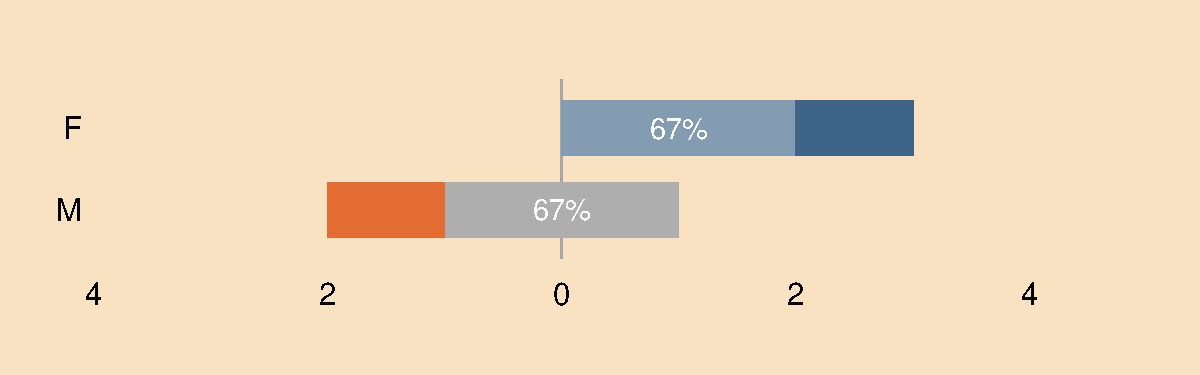
\includegraphics[align=t,trim={5mm 0 5mm 12mm},clip,width=9cm]{fig/pmscareer/ais_support1.pdf}\\

\hdashline 


    I am satisfied with the opportunities I have to discuss promotion opportunities with my line manager/Head of Dept.&
       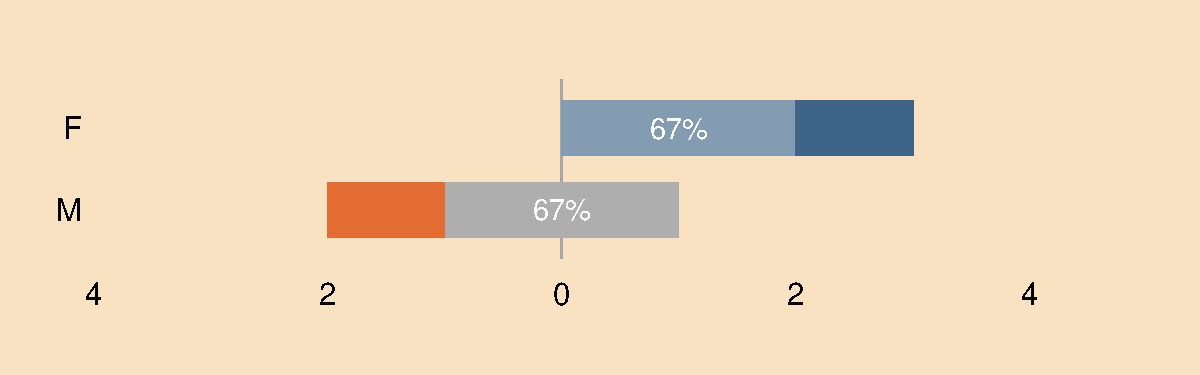
\includegraphics[align=t,trim={5mm 0 5mm 12mm},clip,width=9cm]{fig/pmscareer/ais_support2.pdf}\\

\hdashline

    I have opportunities in the School to get the experience I need in relevant activities to meet the criteria for promotion.&
       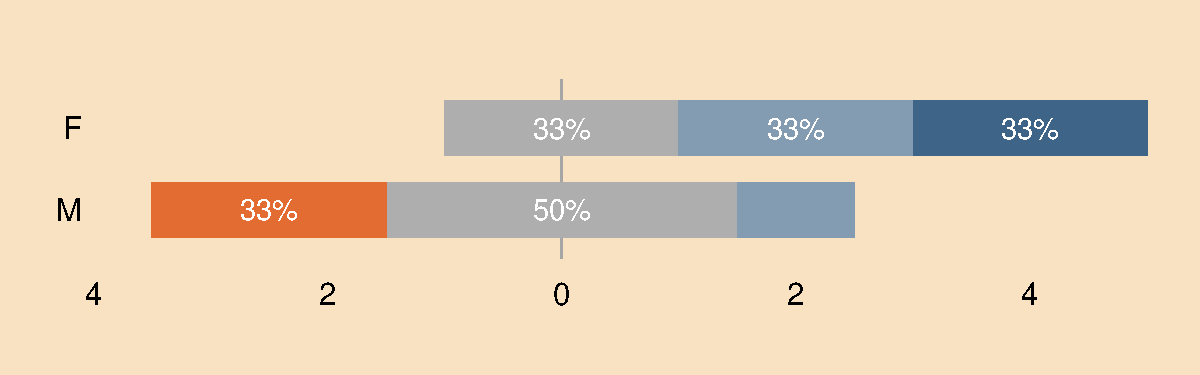
\includegraphics[align=t,trim={5mm 0 5mm 12mm},clip,width=9cm]{fig/pmscareer/ais_support3.pdf}\\

\hdashline 

    I have the support I need in the School to prepare and apply for promotion. &
       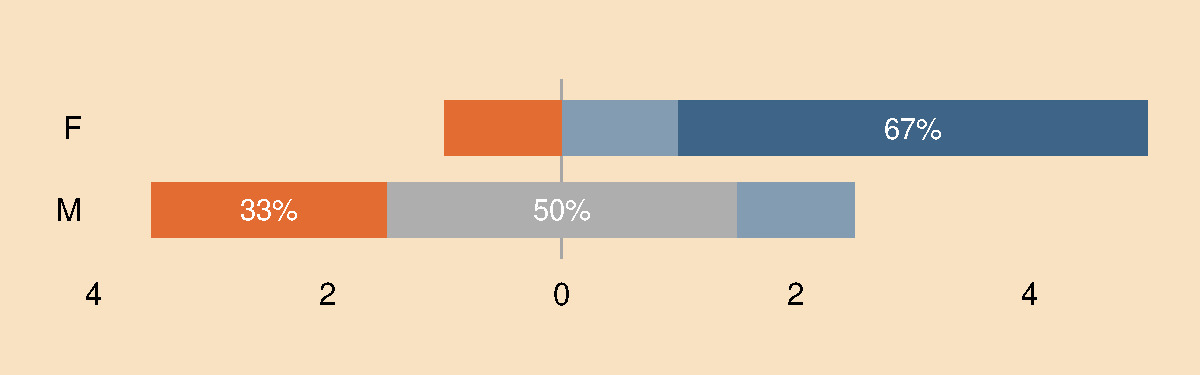
\includegraphics[align=t,trim={5mm 0 5mm 12mm},clip,width=9cm]{fig/pmscareer/ais_support4.pdf}\\


    %% Legend
    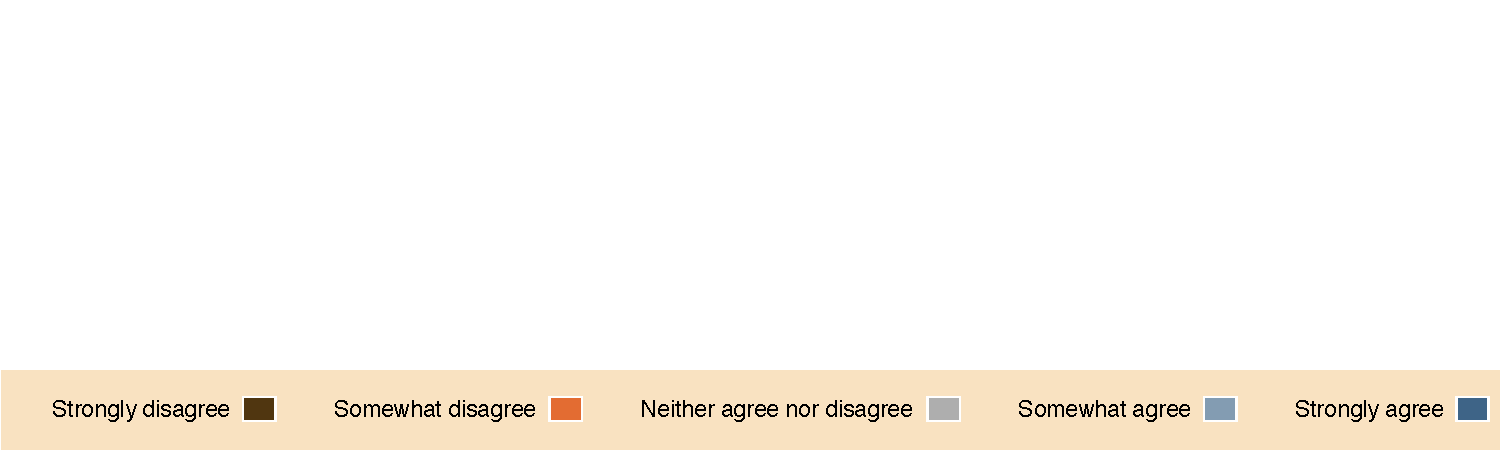
\includegraphics[trim={6mm 0 0 0},clip,width=14.5cm]{fig/legend5col.pdf}
    \end{tabular}

    
\end{figbox}

In the PMS focus group, despite the absence of formal reviews, participants reported strong satisfaction with the opportunities and support available to them to discuss their career/professional development with their line managers:
\begin{myquote}
    ``our line manager is very open to talking about career opportunities but obviously she has a limit. She can’t create promotion opportunities. She’s very supportive and does her best.''
\end{myquote}

\begin{myquote}
    ``There are opportunities to sit down with your line manager and get feedback. Because you know they’re very very open, the door is always open. But I suppose they’re also very restricted in what career path they can lay out for you and incentives to do well without promotional opportunities.''
\end{myquote}

To provide better support for PMS staff in their professional development,  Action~\ref{action:pms:experience} is proposed. 


\begin{actionblock}{\ksspace{}Opportunities for professional experience}{pms:experience}
\actpmsopportunities
\hfill{
    \hypersetup{hidelinks}
    \hyperlink{d8}{\gotoactionsymbol{}}
}
\end{actionblock}


\subsubsection{Information on any additional department-level opportunities for staff to discuss professional development, where different to above (2.e)}

PMS staff have expressed their desire for greater guidance and training for their professional and career development. 
We hope that the restarting of the PDRS (Action~\ref{action:acad:pdrs}) will help in this regard. 




\subsection{Comment and reflect on department engagement with institution-level supports for PMS staff career progression as well as any department-level support available, where different from above (2.\ref{sec:2f}). This should include results from staff consultation presented by gender.}

\begin{tabbox}{!b}
\caption{Training uptake by PMS staff by gender}
\label{tab:training:pms}
\footnotesize 

    
\begin{tabular}{p{2cm}                
                p{9.5cm}
                !{\qquad}
                R{1cm}
                R{1cm}}
    
    \toprule 
    Year  & Course & F & M \\
    \midrule
    
    2017/18 & Mental Health Awareness for Managers & 1 & 1\\
    \cdashline{2-4}
    & Inside Out Mindfulness: Working Mindfully & 0 & 1\\
    \cdashline{2-4}
    & Lean Yellow Belt Training & 0 & 1\\
    \hdashline
    2018/19 & Senior Leadership Development: Aspiring Leaders & 0 & 1\\
    \cdashline{2-4}
    & Innovative Problem Solving & 0 & 1 \\
    \cdashline{2-4}
    & Innovative Problem Solving: Follow Up Session & 0 & 1 \\
    \cdashline{2-4}
    & Lean Yellow Belt Training & 0 & 1 \\
    \cdashline{2-4}
    & Mid Career Financial Planning & 0 & 1 \\
    \cdashline{2-4}
    & Active Listening Skills & 1 & 0 \\
    \cdashline{2-4}
    & The Effective Employee & 5 & 0 \\
    \hdashline
    2019/20 &  Engaging with People who are Angry, Anxious, or Panicked & 1 & 0\\
    \cdashline{2-4}
    & Remote Working Workshop: Employee & 0 & 1 \\
    \cdashline{2-4}
    & Remote Working Workshop: Manager  & 0 & 1 \\
    \cdashline{2-4}
    & The Effective Employee & 1 & 0 \\
    \cdashline{2-4}
    & You and Your MBTI Preferences During Covid-19 & 1 & 0 \\
    \midrule 
    Total & & 10 & 10 \\
    
\bottomrule      
         
\end{tabular}
    
\end{tabbox}

Although CSIT does not operate a formal policy of staff training for career development and progression, it raises awareness of training and progression opportunities. A wide range of training workshops are offered by the university, covering topics such as Teamwork, Leadership Potential, Leadership and Strategic Direction, People Management and Supervision, Management and Delivery of Results, and more.  Table~\ref{tab:training:pms} shows PMS staff engagement with these workshops in the 2017-2020 time period; on balance, there is an even uptake of opportunities among males and females. 




\begin{figbox}{!b}
    \caption{Training supports for PMS career progression}
    %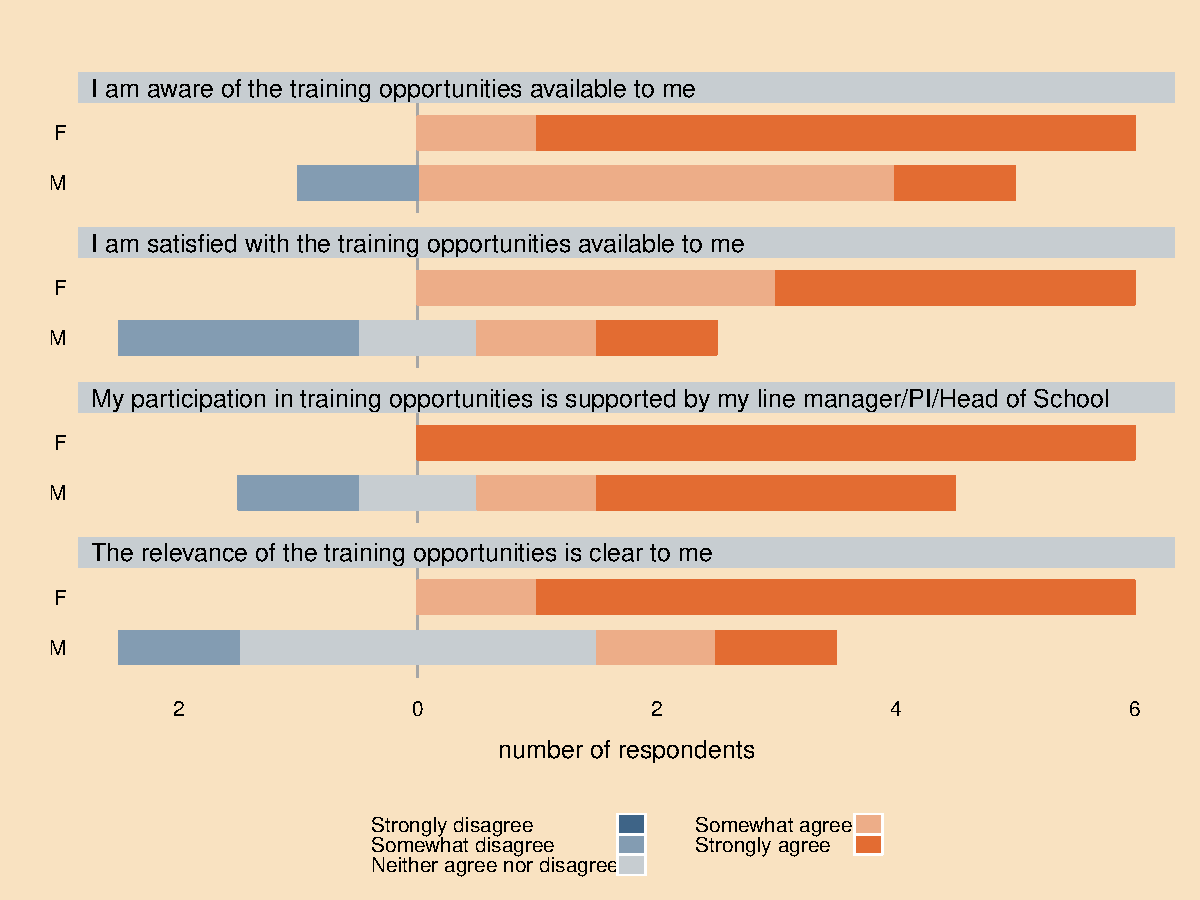
\includegraphics[width=5.5in]{fig/fig234.pdf}
    \label{fig:survey:pms:trainingsupport}

    \sffamily
    \footnotesize
    \raggedright

    \begin{tabular}{M{5cm}
                    !{\qquad}
                    p{8cm}}
    \addlinespace
    I am aware of the training opportunities available to me.&
    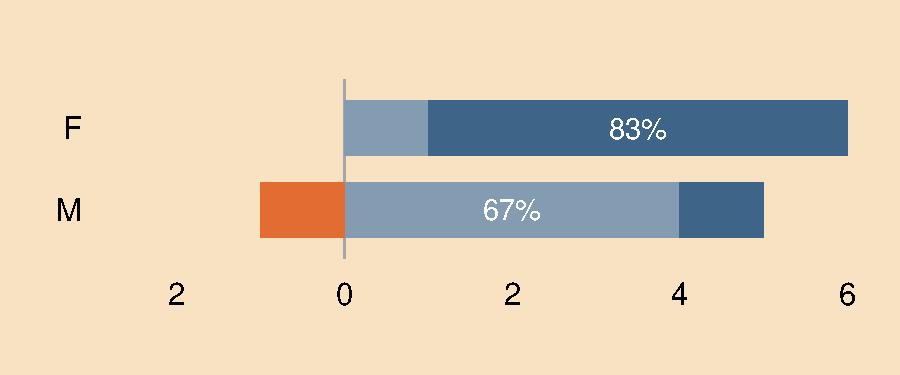
\includegraphics[align=t,trim={5mm 0 0mm 16mm},clip,width=7.5cm]{fig/pmscareer/ais_training1.pdf}\\

\hdashline 

    The relevance of the training opportunities is clear to me.&
       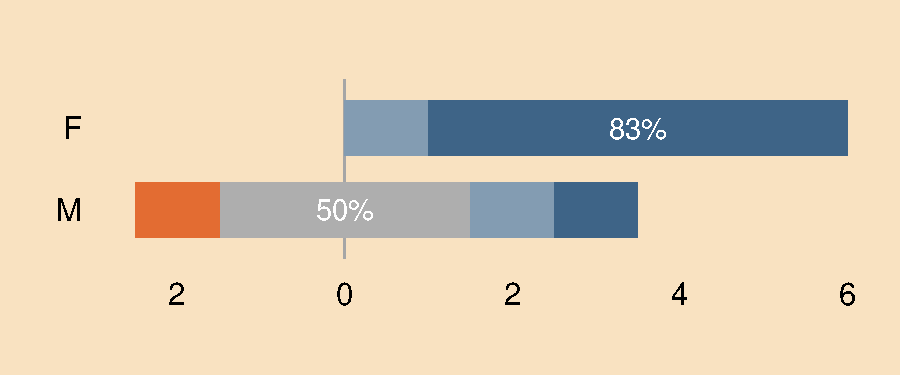
\includegraphics[align=m,trim={5mm 0 0mm 16mm},clip,width=7.5cm]{fig/pmscareer/ais_training2.pdf}\\

\hdashline 

    I am satisfied with the training opportunities available to me.&
       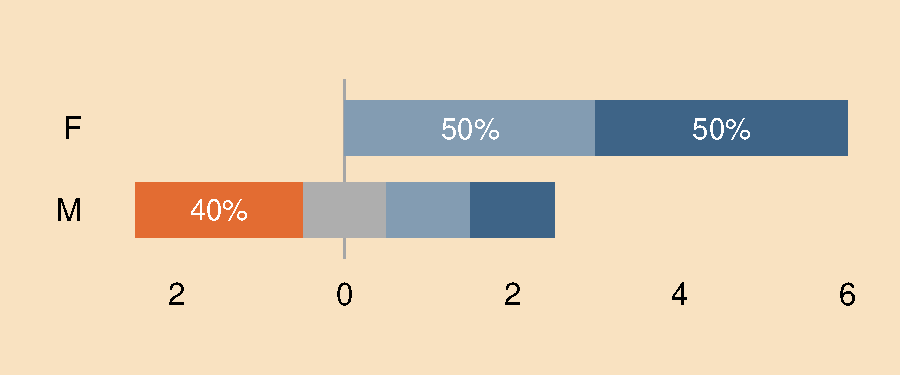
\includegraphics[align=m,trim={5mm 0 0mm 16mm},clip,width=7.5cm]{fig/pmscareer/ais_training3.pdf}\\

\hdashline 

    My participation in training opportunities is supported by my line manager/PI/Head of School. &
       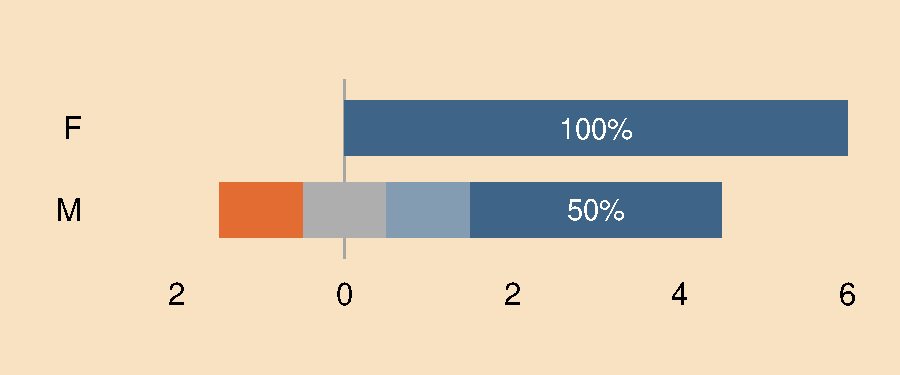
\includegraphics[align=m,trim={5mm 0 0mm 16mm},clip,width=7.5cm]{fig/pmscareer/ais_training4.pdf}\\


    %% Legend
    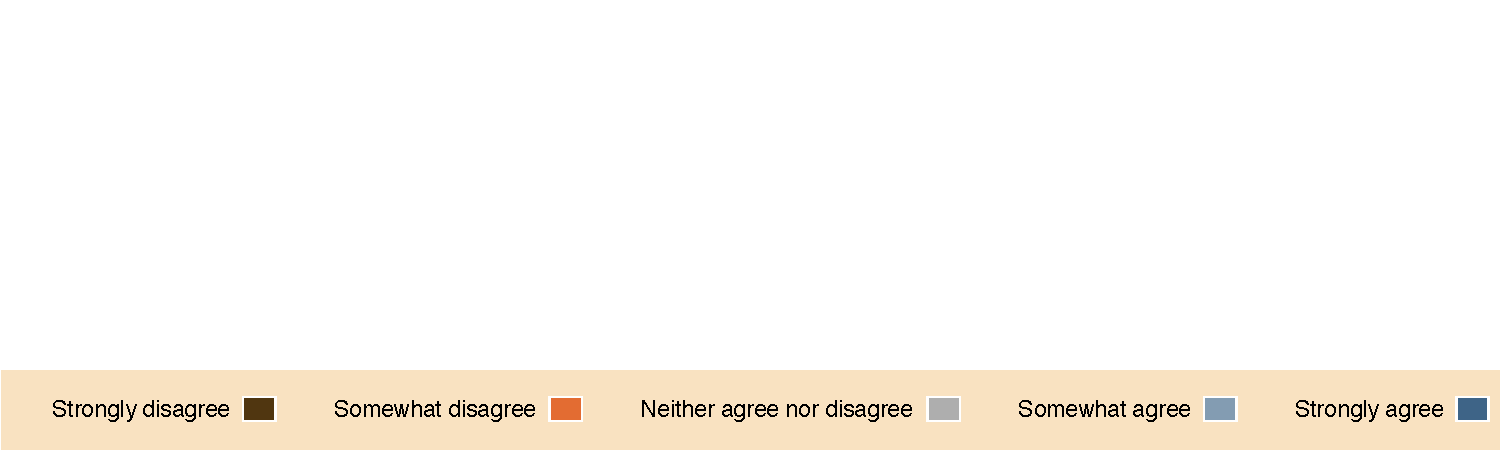
\includegraphics[trim={6mm 0 0 0},clip,width=14.5cm]{fig/legend5col.pdf}
    \end{tabular}
\end{figbox}

PMS staff were asked in the staff survey to reflect on training supports for career progression with responses summarised in Figure~\ref{fig:survey:pms:trainingsupport}. 
Of the 12 PMS respondents, 6 answered this set of questions.  All female respondents were content with the training supports available. The male respondents expressed some minor discontentment. 



\subsection{Comment and reflect on how workload is distributed and managed. This should include information on how the breadth of professional, managerial and support roles and responsibilities are captured in workload planning and allocation and results from staff consultation presented by gender.}

\begin{figbox}{!b}
\caption{Workload distribution, before Covid-19 and during, by gender}
\label{fig:survey:pms:worklife}
    %%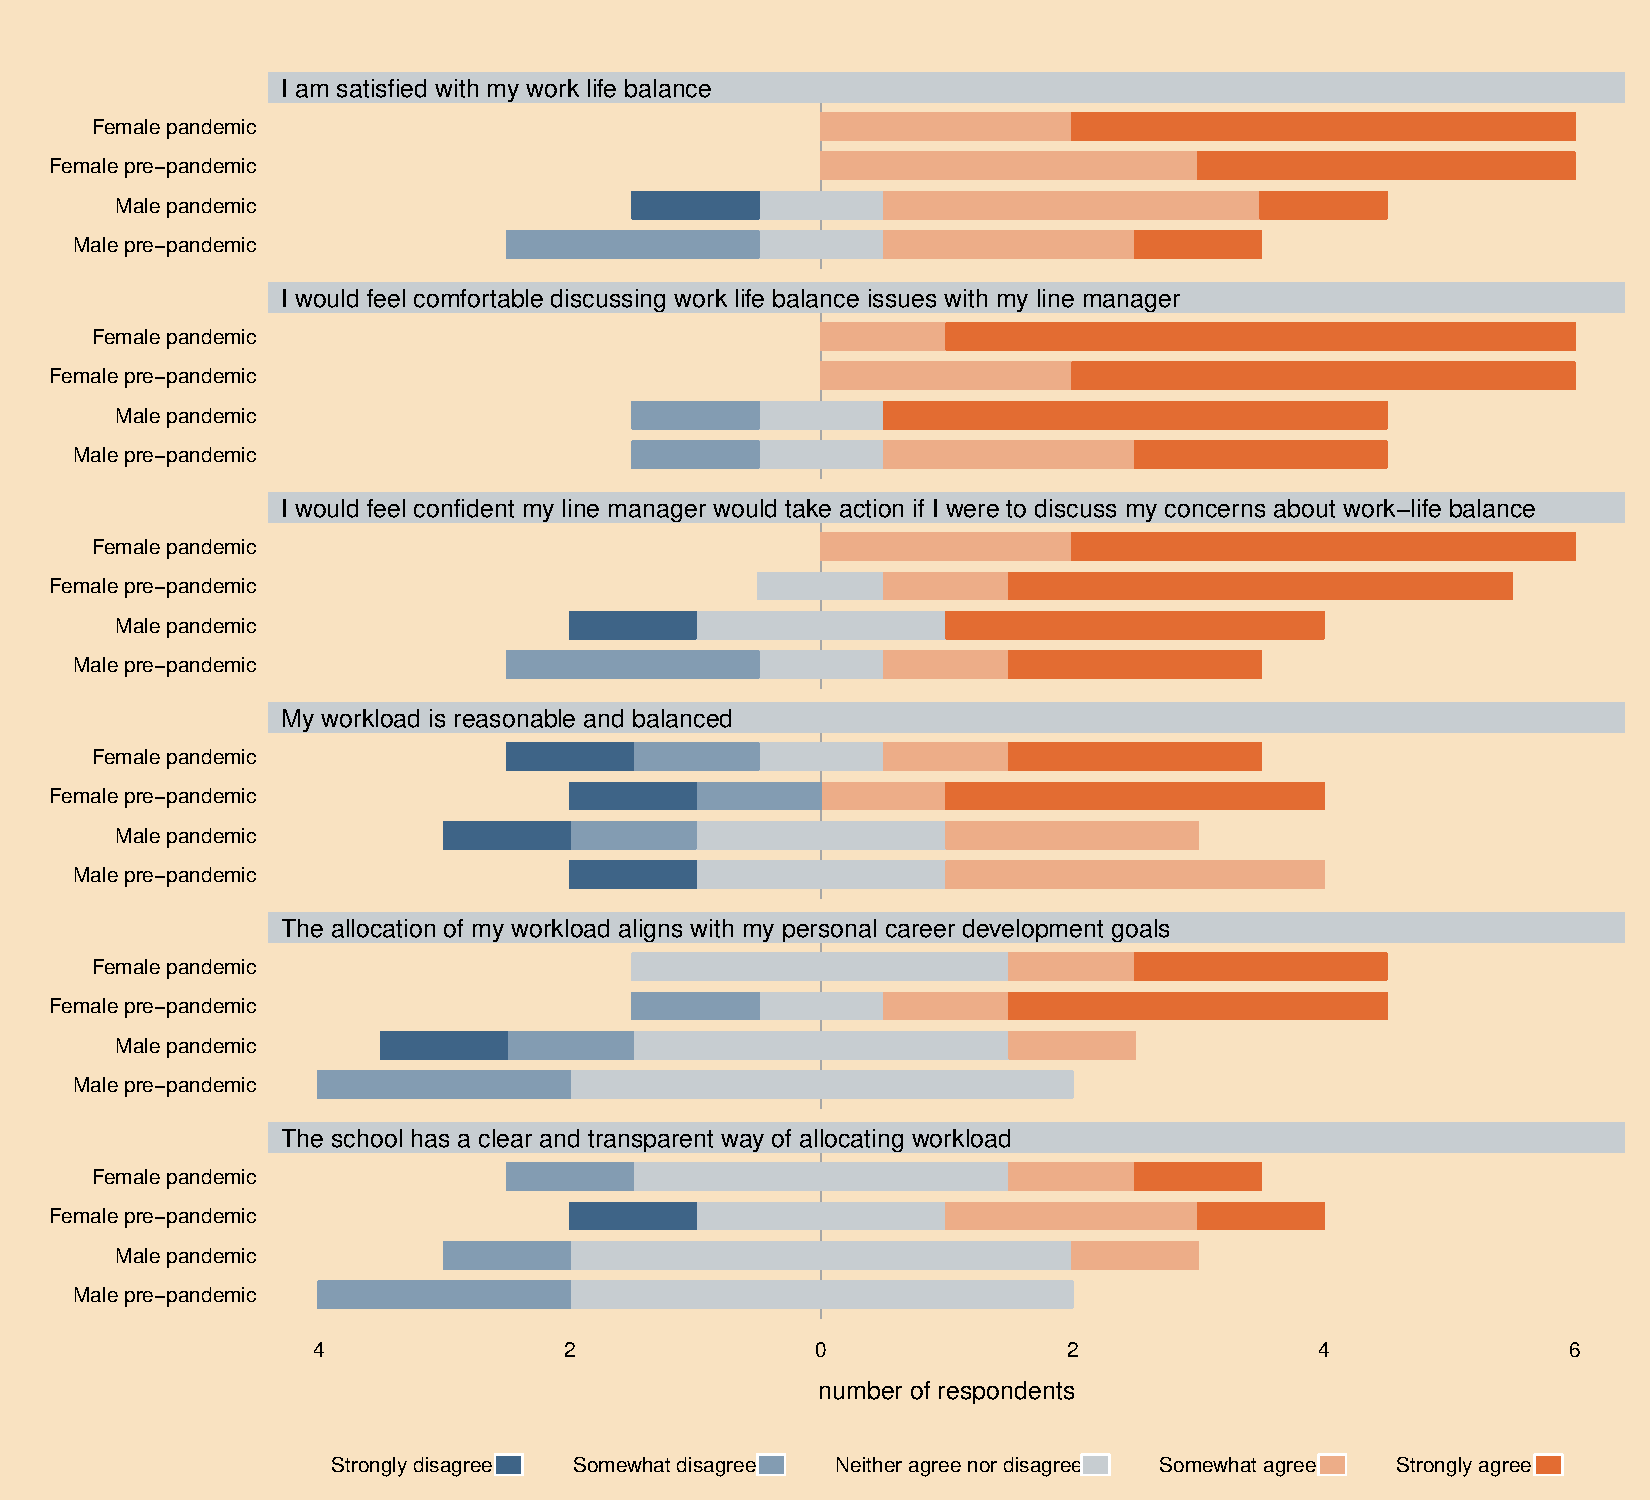
\includegraphics[width=5.5in,trim={0 0 0 0},clip]{fig/pmsworkload_worklife_bal.pdf}
    %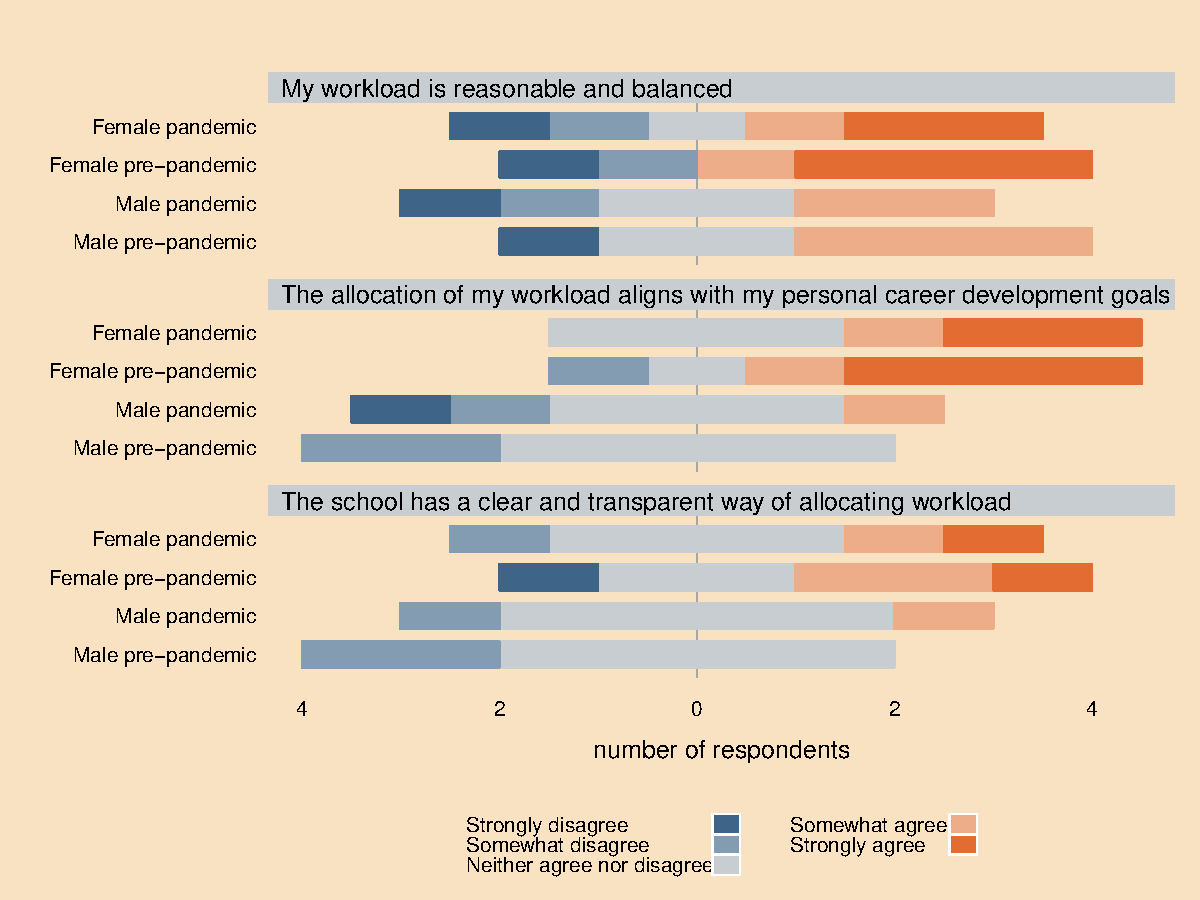
\includegraphics[width=5.5in,trim={0 0 0 0},clip]{fig/pmsworkload.pdf}
    
    \sffamily
    \footnotesize
    \raggedright

    \begin{tabular}{P{4cm}
                    !{\quad}
                    p{10cm}}
    \addlinespace
    My workload is reasonable and balanced (pre-Covid-19).&
    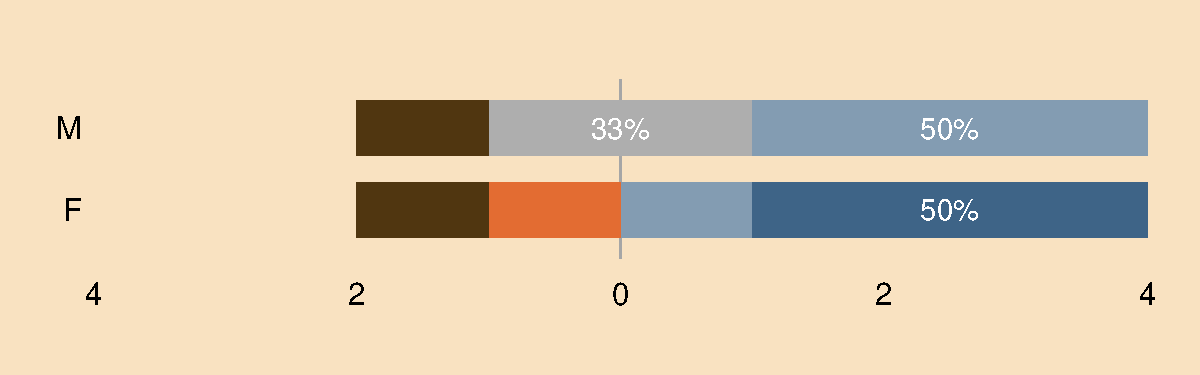
\includegraphics[align=t,trim={5mm 20mm 0mm 12mm},clip,width=9cm]{fig/pmscareer/ais_workload1a.pdf}\\

    %My workload is reasonable and balanced (during Covid-19).
    As above, during Covid-19.
    &
       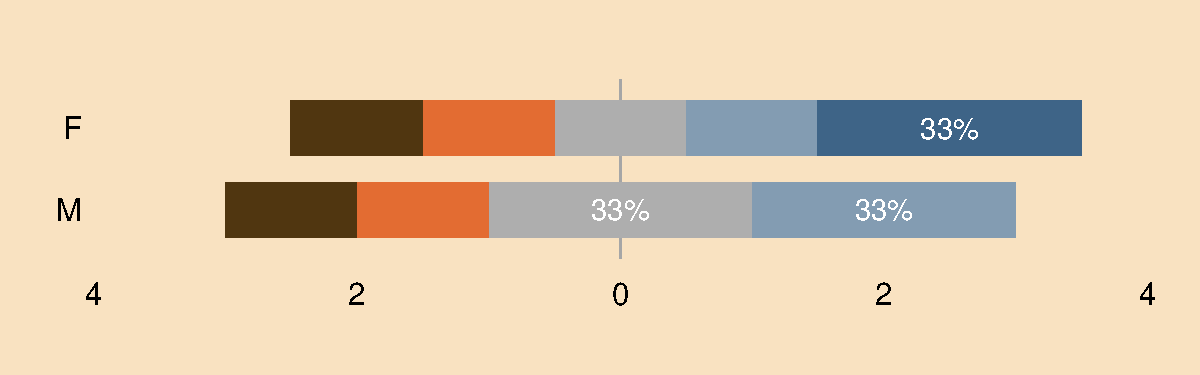
\includegraphics[align=t,trim={5mm 0mm 0mm 16mm},clip,width=9cm]{fig/pmscareer/ais_workload1b.pdf}\\

\hdashline
\addlinespace 
    \multirow{2}{=}{The allocation of my workload aligns with my personal career development goals (pre-Covid-19).\\[5mm] As above, during Covid-19.} &
       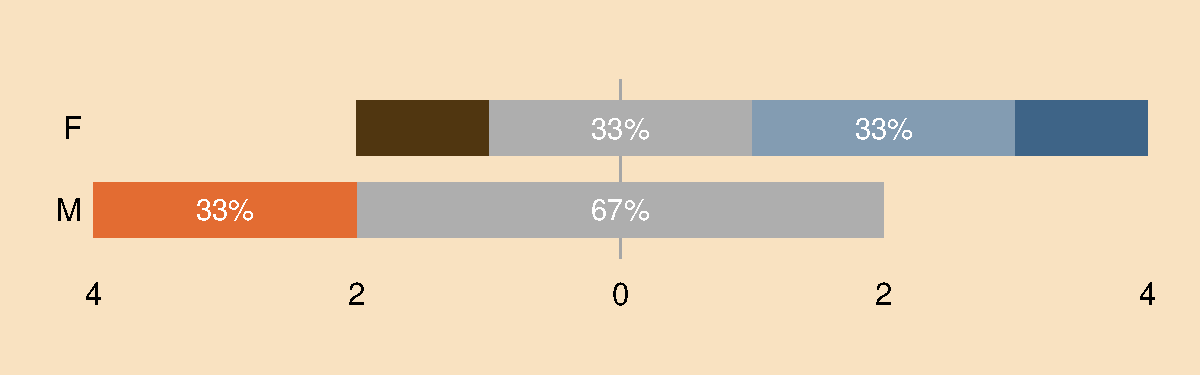
\includegraphics[align=t,trim={5mm 20mm 0mm 12mm},clip,width=9cm]{fig/pmscareer/ais_workload2a.pdf}\\

    %The allocation of my workload aligns with my personal career development goals (during Covid-19). 
    
    &
       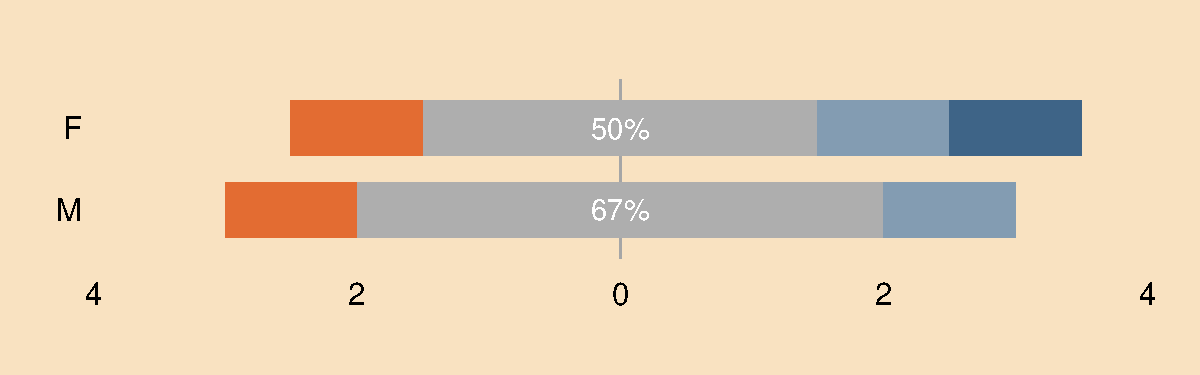
\includegraphics[align=t,trim={5mm 0mm 0mm 16mm},clip,width=9cm]{fig/pmscareer/ais_workload2b.pdf}\\

\hdashline
\addlinespace 
    \multirow{2}{=}{The school has a clear and transparent way of allocating workload (pre-Covid-19).\\[5mm] As above, during Covid-19.} &
       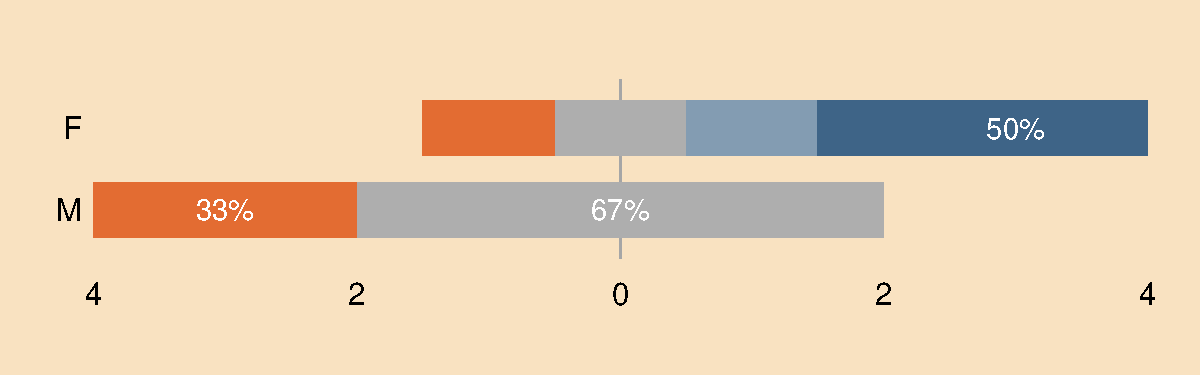
\includegraphics[align=t,trim={5mm 20mm 0mm 12mm},clip,width=9cm]{fig/pmscareer/ais_workload3a.pdf}\\

    %The school has a clear and transparent way of allocating workload (during Covid-19). 
    
    &
       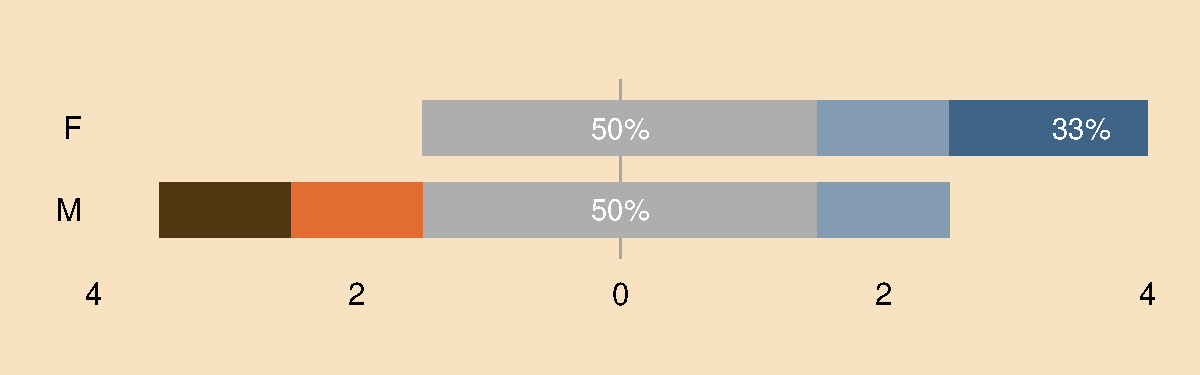
\includegraphics[align=t,trim={5mm 0mm 0mm 16mm},clip,width=9cm]{fig/pmscareer/ais_workload3b.pdf}\\

    %% Legend
    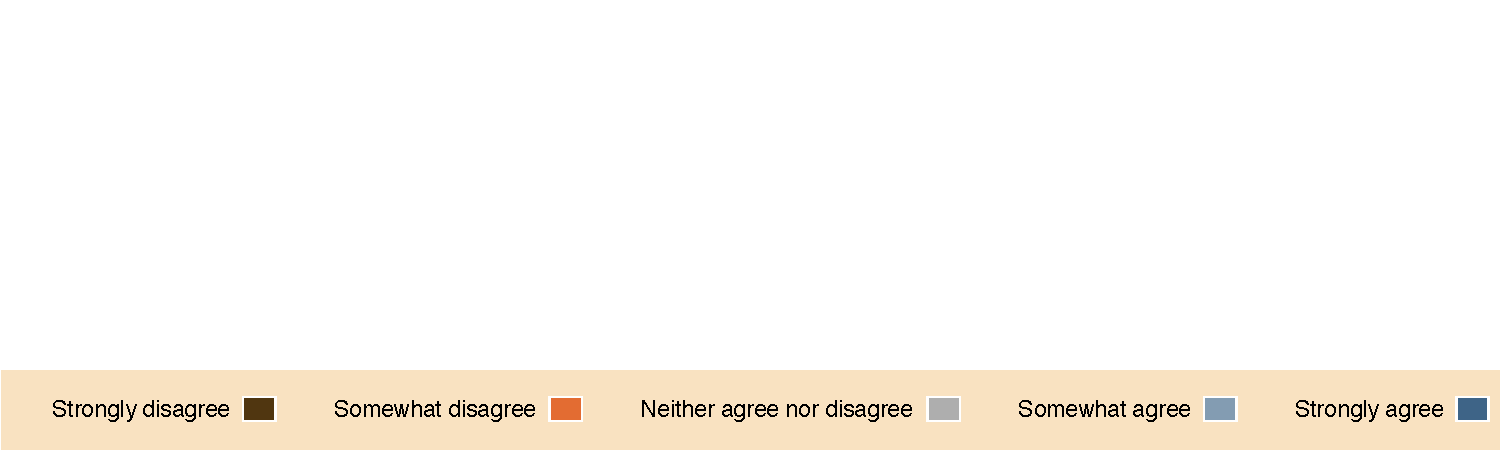
\includegraphics[trim={6mm 0 0 0},clip,width=14.5cm]{fig/legend5col.pdf}
    \end{tabular}

\end{figbox}

Non-research PMS staff workload is managed by the School Manager, subject to their specified responsibilities. The administrative support workload is distributed across
several categories, including academic support, outreach and student recruitment, finance, HR, and health and safety.
Workload is managed by the Computing Systems Manager based on function and matched to the expertise of the staff member.
Functions include IT support, core systems/services, and teaching support.



The workload of the research PMS staff is managed by the general manager of one of the research centres (Table~\ref{tab:researchcentres}), or by a specific \ac{PI} in the case of smaller research units. 



PMS staff were asked to reflect on their workload allocation (Figure~\ref{fig:survey:pms:worklife}), if it was transparently allocated and if it aligned with their career goals.
Generally, the female staff had no opinion or were happy (one was not). The male staff members were marginally less satisfied. 






The pandemic had some influence on people's workload, as reflected in the comments: 
\begin{myquote}
``my workload seems to have increased as many more formal meetings.''
\end{myquote}
\begin{myquote}
``If anything, the workload has increased considerably in the past 16 months.''
\end{myquote}
\begin{myquote}
``Work is more intense since March 12 2020 [the date of the first Covid-19 lockdown]''
\end{myquote}




